\subsection{Sprachsynthese}

\subsubsection*{Benutzeroberfläche}

Erweiterung Inbox um T2S Icon. \\
Erweiterung Admin UI um Checkbox. \\
Zusätzlich Configuration Page mit preferences. \\

\subsubsection*{Konfiguration}

Erweiterung NotificationType um ein boolean Flag für isTextToSpeech.
Wenn Aktiviert, wird Benachrichtigung bei Empfang vorgelesen.

Weiter wird auf dem NotificationType ein Feld version hinzugefügt.
Damit soll die aktuelle Version des NotificationType verfolgt werden.
Wird eine Änderung am NotificationType persisteirt, wird die Version entsprechend angepasst.
Sowohl das Flag isTextToSpeech als auch das version Property werden neu beim Versenden von Benachrichtigungen mitgegeben.

Text To Speech kann auf Client Seite dekativiert werden.
Ist es deaktiviert, werden keine Benachrichtigungen vorgelesen.
Audio Signal, dass Benachrichtung empfangen wurde ertönt aber trotzdem.
Keine zusätzlichen Endpoints am Cloud Service nötig. \\

\begin{figure}[h]
    \centering
    \begin{minipage}[b]{0.75\textwidth}
        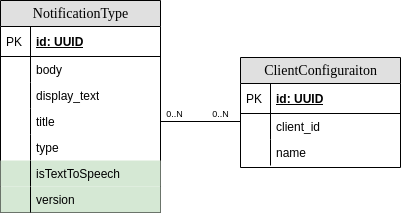
\includegraphics[width=\textwidth]{/home/joshua/FHNW/dev/IP6/IP6_Bachelorarbeit_Bericht_Cloudbasiertes_Praxisrufsystem/src/graphics/diagramms/erd_t2s_v01.drawio}
        \caption{ERD Ausschnitt - Konfiguration Sprachsynthese}
    \end{minipage}
\end{figure}



\clearpage

\subsection*{Laufzeitsicht}

Empfang und Versenden gleich wie bei IP5.
Benachrichtigung enthält zudem neu Flag ob T2S gebraucht werden soll.
Wenn ja, wird Vorlesen an T2S Service delegiert.

\begin{figure}[h]
    \centering
    \begin{minipage}[b]{0.9\textwidth}
        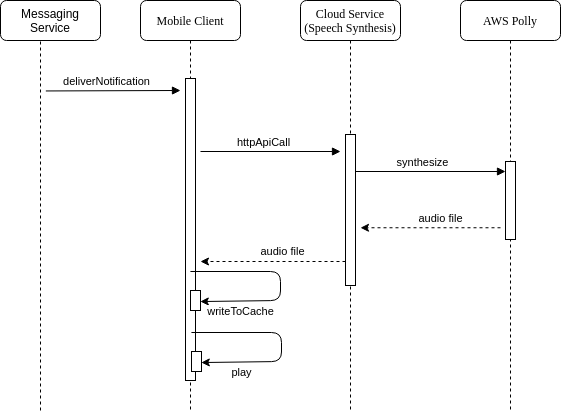
\includegraphics[width=\textwidth]{graphics/diagramms/Sequence_Speech_Synth_V01}
        \caption{Ablauf Benachrichtigung empfangen}
    \end{minipage}
\end{figure}

\clearpage
